%%%%%%%%%%%%%%%%%%%% author.tex %%%%%%%%%%%%%%%%%%%%%%%%%%%%%%%%%%%
%
% sample root file for your "contribution" to a contributed volume
%
% Use this file as a template for your own input.
%
%%%%%%%%%%%%%%%% Springer %%%%%%%%%%%%%%%%%%%%%%%%%%%%%%%%%%


% RECOMMENDED %%%%%%%%%%%%%%%%%%%%%%%%%%%%%%%%%%%%%%%%%%%%%%%%%%%
\documentclass[graybox]{svmult}

% choose options for [] as required from the list
% in the Reference Guide

\usepackage{mathptmx}       % selects Times Roman as basic font
\usepackage{helvet}         % selects Helvetica as sans-serif font
\usepackage{courier}        % selects Courier as typewriter font
\usepackage{type1cm}        % activate if the above 3 fonts are
                            % not available on your system
%
\usepackage{makeidx}         % allows index generation
\usepackage{graphicx}        % standard LaTeX graphics tool
                             % when including figure files
\usepackage{multicol}        % used for the two-column index
\usepackage[bottom]{footmisc}% places footnotes at page bottom

% see the list of further useful packages
% in the Reference Guide

\makeindex             % used for the subject index
                       % please use the style svind.ist with
                       % your makeindex program

%%%%%%%%%%%%%%%%%%%%%%%%%%%%%%%%%%%%%%%%%%%%%%%%%%%%%%%%%%%%%%%%%%%%%%%%%%%%%%%%%%%%%%%%%

\begin{document}

\title*{Incorporating Expert Knowledge in Structural Equation Models: Applications in Psychological Research}
\titlerunning{Incorporating Expert Knowledge in Structural Equation Models}
\subtitle{\emph{Integrare il Parere degli Esperti con i Modelli di Equazioni Strutturali: Applicazioni nella Ricerca Psicologica}}
\author{Gianmarco Alto\`e, Claudio Zandonella Callegher,  Enrico Toffalini and Massimiliano Pastore}
% Use \authorrunning{Short Title} for an abbreviated version of
% your contribution title if the original one is too long
\authorrunning{G. Alto\`e, C. Zandonella Callegher,  E. Toffalini and M. Pastore}
\institute{
Gianmarco Alto\`e \at Department of Developmental Psychology and Socialisation, University of Padova \\ \email{gianmarco.altoe@unipd.it}
\and Claudio Zandonella Callegher \at Department of Developmental Psychology and Socialisation, University of Padova \\ \email{claudio.zandonellacallegher@phd.unipd.it}
\and Enrico Toffalini \at Department of General
Psychology, University of Padova \\ \email{enrico.toffalini@yahoo.it}
\and Massimiliano Pastore \at Department of Developmental Psychology and Socialisation, University of Padova  \\
 \email{massimiliano.pastore@unipd.it}
}
%
% Use the package "url.sty" to avoid
% problems with special characters
% used in your e-mail or web address
%
\maketitle

\abstract{The abstract should be written in English and in Italian, each paper should be preceded by an abstract (no more than 10 lines long) that summarizes the content. Please insert your abstract here.}
\abstract{\emph{Abstract in Italian}}
\keywords{Expert elicitation, Informative Priors, Structural Equation Models (SEM), Small sample sizes, Psychological research}

\section{Introduction}
\label{sec:1}

\emph{Structural Equation Modeling} (SEM) encompasses  a range of multivariate statistical techniques as, for example, confirmatory factor analysis, path analysis, or latent growth modeling. Generally, SEMs are composed of two parts: a \emph{measurement model} and a \emph{structural model} (see Fig.~\ref{fig:figure1}).   The measurement model defines unobserved constructs (\emph{latent variables}, represented in Fig.~\ref{fig:figure1} as circles) according to a set of measured outcomes (\emph{observed variables}, represented in Fig.~\ref{fig:figure1} as squares), whereas the structural model describes the relationships between latent variables.

\begin{figure}[t]
	\sidecaption
	\label{fig:figure1}
	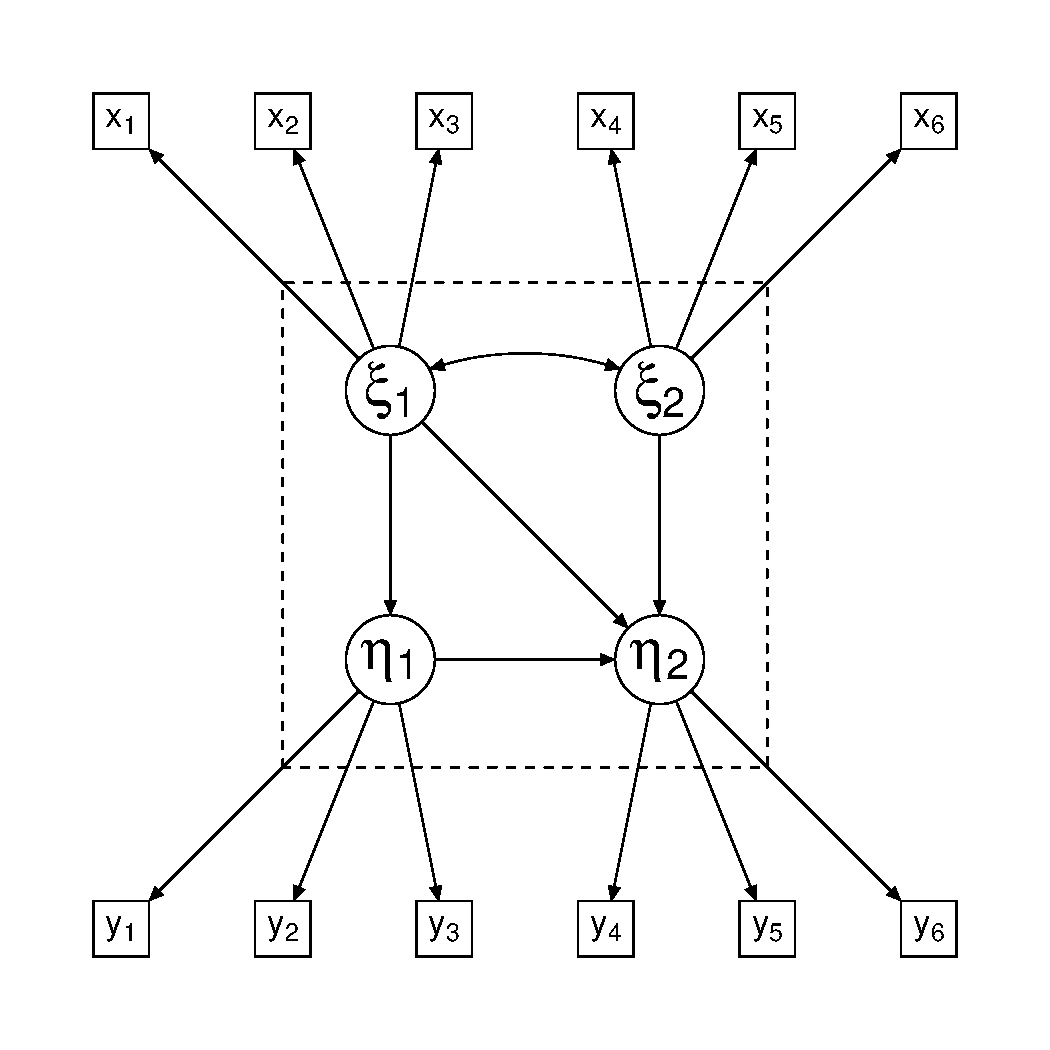
\includegraphics[width = .50\textwidth]{figure/figure1}
	\caption{A typical structural equation model with a structural part (within the dashed box) and multiple measurement models. Circles represent latent variables; rectangles represent observed variables.}
\end{figure}

In SEM, parameters are estimated by minimizing a discrepancy function between the sample covariance matrix and the covariance matrix implied by the model. Considering the covariance structure (instead of modeling all the observed data) allows to model complex relations between variables taking into account also the  measurement error.

% Common applications of SEMs include \emph{factor analysis}, which reduces correlated observed variables into a smaller number of underlying variables, \emph{path analysis}, where only the relations among latent variables are evaluated without considering the measurement model, and \emph{latent growth models}, used to estimate growth trajectories.

Given their great flexibility, SEMs are widely used in psychology for various purposes such as validating psychological tests and questionnaires or evaluating hypotheses and theoretical models that involve complex relations between different latent psychological constructs.

However, as the complexity of the model increases, more data are required to obtain accurate parameter estimates and model fit statistics \cite{wolfSampleSizeRequirements2013}. Recent concerns about the replicability of psychological results have raised awareness on the importance of properly define an adequate sample size \cite{ioannidisWhyMostPublished2005, opensciencecollaborationEstimatingReproducibilityPsychological2015}.  Nevertheless, in many research settings, the number of participants may be limited due to financial restriction, strict inclusion criteria, or clinical samples. In the case of small sample sizes, appropriate statistical techniques are required to enhance the reliability of the results.

Often in the literature, the Bayesian approach is suggested over frequentist estimation when limited data are available \cite{mcneishUsingBayesianMethods2016a}.  In the context of small sample, the inclusion of prior information can help in the parameter estimation, but researchers have to carefully consider priors choice, as estimates are highly sensitive to the prior specification (or misspecification).

The use of Bayesian statistical approach is increasing and availability of softwares, such as R-package \texttt{blavaan} \cite{merkleBlavaanBayesianStructural2018},  provide researchers with flexible tools for estimating even Bayesian structural equation models. However, most of the studies are unlikely to carefully consider priors choices, and often they rely on default software prior settings. A recent review, considering the performance of Bayesian estimation for structural equation models with small sample sizes, underlined that the use of diffuse default priors can result in severely biased estimates, and this bias can be decreased only by incorporating informative priors \cite{smidBayesianFrequentistEstimation2020}. Thus, authors warn against the use of \emph{naive prior} (i.e., diffuse default priors) when samples are small, and encourage researchers to incorporate \emph{thoughtful priors} (i.e., informative priors).

Informative priors allow researchers to include in the analysis relevant knowledge in the field, such as previous studies results, meta-analyses or expert opinions. Priors choice should be clearly discussed and researchers are required to evaluate the generalizability of external information to the specific characteristics of their study. When the number of available studies is limited or their quality is judged not adequate, relying only on previous results in the literature could be misleading. In these cases, researchers could consider to include opinions of experts as well. On the base of their experience in the field, experts can evaluate relevant information and help researchers in the definition of a plausible range of values and prior choices.

The remainder of this article is structured as follows. In Sec.~\ref{sec:expert_elicitation}, we briefly consider how informative priors can be defined according to experts' opinions. In Sec.~\ref{sec:simulation}, we present a simulation study to evaluate the influence of different prior specifications in the case of structural equation models with small sample size, considering an applied example of a mediation model in psychology. Finally, in Sec.~\ref{sec:dicussion}, we discuss the obtained results highlighting limits and future developments of using expert knowledge with structural equation models in the case of  small sample sizes.

\section{Expert knowledge elicitation}
\label{sec:expert_elicitation}

\emph{Elicitation} is a structured procedure that allows experts to express their knowledge and uncertainty about quantities of interest in the form of probability distributions \cite{ohaganExpertKnowledgeElicitation2019}. Elicitation can be used to define informative priors according to  experts' judgement.

Different elicitation methods have been proposed in the literature such as the \emph{Cooke protocol} \cite{cookeExpertsUncertaintyOpinion1991}, the \emph{Delphi method} \cite{roweDelphiTechniqueForecasting1999} or the \emph{SHELF protocol} \cite{oakleySHELFSheffieldElicitation2016}. The common aim of these methods is to make a subjective judgement as much objective as possible by limiting potential sources of bias, forcing the experts to carefully reason about the answer, and by documenting and transparently reporting all the procedure. In general, elicitation is composed of three phases \cite{ohaganUncertainJudgementsEliciting2006}:

\begin{enumerate}
	\item{\emph{Preparation and training} - experts are informed about  the aim of the elicitation and the parameters and quantities to elicit are clearly defined. All the relevant information about the topic of interest is collected and made available to experts. Next, experts are trained to make probabilistic judgements and they are familiarize with the elicitation process in a practice example to avoid misunderstandings. }
	\item{\emph{Individual judgements elicitation} - experts express their own judgement for each parameter or quantity of interest according to the elicitation technique they were trained before. Two of the main elicitation technique are the \emph{quartile method} and the \emph{roulette method}. In the former, experts provide values for the medians  and the quartile of the distribution according to their expectation. In the latter, the range of plausible values is divided into different intervals and the experts can place a given number of tokens to allocate probabilities according to  their expectation.}
	\item{\emph{Aggregation of individual judgements} - the individual judgements of the different experts are aggregate to obtain a unique final distribution. The two principal approaches are \emph{mathematical  aggregation}, where distributions are combined mathematically according to a pooling rule, and \emph{behavioral aggregation}, where experts are required to discuss together their opinions and reach a consensus judgement from which the aggregate distribution is obtained.}
\end{enumerate}

Elicitation methods differ in the solutions adopted during each phase and in the emphasis given to the different aspects of the elicitation. For example, in the Cooke protocol experts are not required to meet each other. Experts return a form with their individual answer and mathematical aggregation is used to summarize the results. In the SHELF protocol, instead, much more emphasis is given to the collaboration between experts. After the  individual judgments, experts discuss and share their opinions to then reach a common final answer.

Researchers willing to conduct an elicitation process should evaluate the pros and cons of each methods considering their own needs and constraints such as availability of experts, the possibility to group experts together, number of quantities to elicit or financial and time constraints.

\section{Simulation}
\label{sec:simulation}

To evaluate the influence of different prior specifications in the case of structural equation models with small sample size, we considered a mediation model from \cite{sellaPersonalityTraitsSleep2020}  presented in Fig.~\ref{fig:model_example}. The study evaluated the relationship between participants' self-reported sleep quality, personality characteristics, and negative beliefs about sleeping problems. In particular, the study found that the association between participants' tendency to experience distress and become anxious (\emph{Neuroticism}) and self-reported sleep quality (\emph{Sleep quality}) is small ($\beta_3=-.13$).  A stronger association is given  by the mediation role of the participants tendency to have negative thoughts about sleeping difficulties (\emph{Metacognitive thoughts}). In other words, people with higher levels of distress and anxiety tend to have dysfunctional beliefs and attitudes about sleep ($\beta_1=.20$) that, in turns, induce them to perceive and report a worse-quality sleep ($\beta_2=-.36$).

\begin{figure}[b]
	\sidecaption
	\label{fig:model_example}
	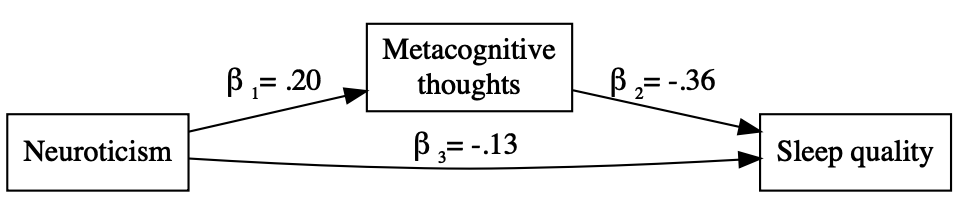
\includegraphics[width = .64\textwidth]{figure/Plot_example_model}
	\caption{Mediation model from \cite{sellaPersonalityTraitsSleep2020}. Neuroticism is not directly associated to sleep quality but is mediated by metacognitive thoughts.}
\end{figure}

\subsection{Simulation details}

The simulation was carried in \texttt{R} version 3.X.X \cite{rcoreteamLanguageEnvironmentStatistical2018} using packages \texttt{lavaan} \cite{rosseelLavaanPackageStructural2012} and \texttt{blavaan} \cite{merkleBlavaanBayesianStructural2018}.

In the simulation, we  considered as parameters of interest the regression coefficients ($\beta_1,\ \beta_2,\ \beta_3$) of the model presented above. We compared the performance of Maximum Likelihood (ML) estimation and Bayesian estimation under different sample size (i.e., 20, 50, 100, 500). In the current case, sample sizes below 100 can be considered small, but they are. Wherase 500 would be a more appropriate sample size and is considered as reference

 using three different prior distribution specifications. The different prior specifications are listed below and represented in Fig.~\ref{fig:prior}.

\begin{enumerate}
	\item{\textit{Default prior} -  in \texttt{blavaan}, default priors for regression coefficients are $N(0,10)$}. These priors are diffuse over a wide range of values (95\% CI\ [-19.6;\ 19.6]) and are intended to be non-informative.
	\item{\textit{Reasonable prior} - the priors are $\beta_1\sim N(.20,\ .50)$, and  $\beta_{2;3}\sim N(-.20,\ .50)$, that correspond, respectively, to a 95\% CI of  [-0.78;\ 1.18] and  [-1.18; 0.78]. These priors are moderately informative, they are intended to exclude excessively large values that are not reasonable within psychology research. Moreover, the mean of each prior distribution is slightly moved above or below zero to reflect the direction of the main results in the literature for each relation.}
 	\item{\textit{Experts prior} - the priors are $\beta_1\sim N(.20,\ .20)$,  $\beta_{2}\sim N(-.40,\ .20)$}, and $\beta_3\sim N(-.20,\ .20)$. These priors are intended to be highly informative, they are intended to represent experts judgement of the quantities of interest according to previous results in the literature and their experience in the field.
\end{enumerate}

\begin{figure}[b]
	\sidecaption
	\label{fig:prior}
	\includegraphics[width = .64\textwidth]{figure/plot_prior}
	\caption{Prior distribution in the three different settings.}
\end{figure}

\section{Discussion and conclusions}

\label{sec:dicussion}

\clearpage
\bibliographystyle{spmpsci.bst}
\bibliography{SIS_2020.bib}


% uncomment the following line to insert reference (dos not work in R-studio, copile with another LaTeX editor)
%%%%%%%%%%%%%%%%%%%%%%%%% referenc.tex %%%%%%%%%%%%%%%%%%%%%%%%%%%%%%
% sample references
% %
% Use this file as a template for your own input.
%
%%%%%%%%%%%%%%%%%%%%%%%% Springer-Verlag %%%%%%%%%%%%%%%%%%%%%%%%%%
%
% BibTeX users please use
% \bibliographystyle{}
% \bibliography{}
%
\biblstarthook{References may be \textit{cited} in the text either by number (preferred) or by author/year.\footnote{Make sure that all references from the list are cited in the text. Those not cited should be moved to a separate \textit{Further Reading} section or chapter.} The reference list should ideally be \textit{sorted} in alphabetical order -- even if reference numbers are used for the their citation in the text. If there are several works by the same author, the following order should be used: 
\begin{enumerate}
\item all works by the author alone, ordered chronologically by year of publication
\item all works by the author with a coauthor, ordered alphabetically by coauthor
\item all works by the author with several coauthors, ordered chronologically by year of publication.
\end{enumerate}
The recommended style for references\footnote{Always use the standard abbreviation of a journal's name according to the ISSN \textit{List of Title Word Abbreviations}.} is depicted in ~\cite{science-contrib, science-online, science-mono, science-journal, science-DOI}.
}

\begin{thebibliography}{99.}%
% and use \bibitem to create references.
%
% Use the following syntax and markup for your references if 
% the subject of your book is from the field 
% "Mathematics, Physics, Statistics, Computer Science"
%
% Contribution 
\bibitem{science-contrib} Broy, M.: Software engineering --- from auxiliary to key technologies. In: Broy, M., Dener, E. (eds.) Software Pioneers, pp. 10-13. Springer, Heidelberg (2002)
%
% Online Document
\bibitem{science-online} Dod, J.: Effective substances. In: The Dictionary of Substances and Their Effects. Royal Society of Chemistry (1999) Available via DIALOG. \\
\url{http://www.rsc.org/dose/title of subordinate document. Cited 15 Jan 1999}
%
% Monograph
\bibitem{science-mono} Geddes, K.O., Czapor, S.R., Labahn, G.: Algorithms for Computer Algebra. Kluwer, Boston (1992) 
%
% Journal article
\bibitem{science-journal} Hamburger, C.: Quasimonotonicity, regularity and duality for nonlinear systems of partial differential equations. Ann. Mat. Pura. Appl. \textbf{169}, 321--354 (1995)
%
% Journal article by DOI
\bibitem{science-DOI} Slifka, M.K., Whitton, J.L.: Clinical implications of dysregulated cytokine production. J. Mol. Med. (2000) doi: 10.1007/s001090000086 
%
\end{thebibliography}

\end{document}
